\begingroup\fontsize{9}{11}\selectfont

\begin{longtable}[t]{llllrrrrrr}
\caption{\label{tab:arbitrary_trend_table}We run a logistic model regressing success against perturb-target distance (relative to image width/height) and perturb box length (relative to image width/height) in the deliberate attack experiment. Longer perturb box length (relative to image width/height) or shorter perturb-target distance (relative to image width/height) cause success rates to significantly increase for all model and attack combinations, except for perturb box length (relative to image width/height) in untargeted attack on Cascade R-CNN. The interaction terms, even when significant, are negligibly close to 0. Table headers are explained in Appendix \ref{app:tab_hdr}.}\\
\toprule
\multicolumn{2}{c}{Group} & \multicolumn{8}{c}{Regression} \\
\cmidrule(l{3pt}r{3pt}){1-2} \cmidrule(l{3pt}r{3pt}){3-10}
 & Attack & term & sig & estimate & std.error & statistic & p.value & conf.low & conf.high\\
\midrule
\addlinespace[0.3em]
\multicolumn{10}{l}{\textbf{YOLOv3}}\\
\hspace{1em} & Vanishing & distance & * & -6.969 & 1.182 & -5.898 & 0.000 & -9.308 & -4.674\\
\cmidrule{3-10}\nopagebreak
\hspace{1em} &  & length & * & 7.744 & 0.453 & 17.110 & 0.000 & 6.873 & 8.648\\
\cmidrule{3-10}\nopagebreak
\hspace{1em} &  & distance * length & * & -15.800 & 3.262 & -4.844 & 0.000 & -22.195 & -9.400\\
\cmidrule{2-10}\nopagebreak
\hspace{1em} & Mislabeling & distance & * & -7.516 & 1.198 & -6.276 & 0.000 & -9.891 & -5.194\\
\cmidrule{3-10}\nopagebreak
\hspace{1em} &  & length & * & 5.962 & 0.354 & 16.853 & 0.000 & 5.277 & 6.664\\
\cmidrule{3-10}\nopagebreak
\hspace{1em} &  & distance * length &  & -3.757 & 2.981 & -1.260 & 0.208 & -9.565 & 2.127\\
\cmidrule{2-10}\nopagebreak
\hspace{1em} & Untargeted & distance & * & -9.214 & 1.496 & -6.157 & 0.000 & -12.205 & -6.335\\
\cmidrule{3-10}\nopagebreak
\hspace{1em} &  & length & * & 2.276 & 0.257 & 8.860 & 0.000 & 1.775 & 2.782\\
\cmidrule{3-10}\nopagebreak
\hspace{1em} &  & distance * length &  & 3.324 & 2.896 & 1.148 & 0.251 & -2.311 & 9.048\\
\cmidrule{1-10}\pagebreak[0]
\addlinespace[0.3em]
\multicolumn{10}{l}{\textbf{SSD}}\\
\hspace{1em} & Vanishing & distance & * & -11.391 & 1.488 & -7.656 & 0.000 & -14.362 & -8.527\\
\cmidrule{3-10}\nopagebreak
\hspace{1em} &  & length & * & 4.449 & 0.281 & 15.841 & 0.000 & 3.903 & 5.004\\
\cmidrule{3-10}\nopagebreak
\hspace{1em} &  & distance * length &  & -2.946 & 2.946 & -1.000 & 0.317 & -8.682 & 2.871\\
\cmidrule{2-10}\nopagebreak
\hspace{1em} & Mislabeling & distance & * & -9.002 & 1.596 & -5.641 & 0.000 & -12.194 & -5.934\\
\cmidrule{3-10}\nopagebreak
\hspace{1em} &  & length & * & 5.846 & 0.303 & 19.286 & 0.000 & 5.257 & 6.446\\
\cmidrule{3-10}\nopagebreak
\hspace{1em} &  & distance * length & * & -13.088 & 3.183 & -4.111 & 0.000 & -19.300 & -6.813\\
\cmidrule{2-10}\nopagebreak
\hspace{1em} & Untargeted & distance & * & -10.046 & 1.760 & -5.710 & 0.000 & -13.580 & -6.679\\
\cmidrule{3-10}\nopagebreak
\hspace{1em} &  & length & * & 3.873 & 0.280 & 13.823 & 0.000 & 3.328 & 4.426\\
\cmidrule{3-10}\nopagebreak
\hspace{1em} &  & distance * length & * & -9.039 & 3.479 & -2.598 & 0.009 & -15.823 & -2.178\\
\cmidrule{1-10}\pagebreak[0]
\addlinespace[0.3em]
\multicolumn{10}{l}{\textbf{RetinaNet}}\\
\hspace{1em} & Vanishing & distance & * & -22.822 & 2.997 & -7.615 & 0.000 & -28.866 & -17.129\\
\cmidrule{3-10}\nopagebreak
\hspace{1em} &  & length & * & 2.657 & 0.333 & 7.978 & 0.000 & 2.008 & 3.313\\
\cmidrule{3-10}\nopagebreak
\hspace{1em} &  & distance * length &  & -10.710 & 6.207 & -1.725 & 0.084 & -22.836 & 1.492\\
\cmidrule{2-10}\nopagebreak
\hspace{1em} & Mislabeling & distance & * & -23.172 & 4.211 & -5.503 & 0.000 & -31.759 & -15.284\\
\cmidrule{3-10}\nopagebreak
\hspace{1em} &  & length & * & 1.352 & 0.411 & 3.293 & 0.001 & 0.552 & 2.162\\
\cmidrule{3-10}\nopagebreak
\hspace{1em} &  & distance * length &  & 3.035 & 8.178 & 0.371 & 0.711 & -12.833 & 19.200\\
\cmidrule{2-10}\nopagebreak
\hspace{1em} & Untargeted & distance & * & -23.262 & 2.438 & -9.540 & 0.000 & -28.144 & -18.587\\
\cmidrule{3-10}\nopagebreak
\hspace{1em} &  & length & * & 2.805 & 0.310 & 9.056 & 0.000 & 2.203 & 3.417\\
\cmidrule{3-10}\nopagebreak
\hspace{1em} &  & distance * length & * & 36.482 & 4.181 & 8.726 & 0.000 & 28.422 & 44.811\\
\cmidrule{1-10}\pagebreak[0]
\addlinespace[0.3em]
\multicolumn{10}{l}{\textbf{Faster R-CNN}}\\
\hspace{1em} & Vanishing & distance & * & -31.003 & 3.728 & -8.317 & 0.000 & -38.489 & -23.891\\
\cmidrule{3-10}\nopagebreak
\hspace{1em} &  & length & * & 2.099 & 0.353 & 5.954 & 0.000 & 1.413 & 2.795\\
\cmidrule{3-10}\nopagebreak
\hspace{1em} &  & distance * length &  & -0.776 & 7.406 & -0.105 & 0.917 & -15.251 & 13.769\\
\cmidrule{2-10}\nopagebreak
\hspace{1em} & Mislabeling & distance & * & -27.655 & 4.100 & -6.745 & 0.000 & -35.955 & -19.909\\
\cmidrule{3-10}\nopagebreak
\hspace{1em} &  & length & * & 1.000 & 0.384 & 2.606 & 0.009 & 0.253 & 1.757\\
\cmidrule{3-10}\nopagebreak
\hspace{1em} &  & distance * length &  & 9.942 & 7.822 & 1.271 & 0.204 & -5.291 & 25.353\\
\cmidrule{2-10}\nopagebreak
\hspace{1em} & Untargeted & distance & * & -29.452 & 2.752 & -10.702 & 0.000 & -34.974 & -24.189\\
\cmidrule{3-10}\nopagebreak
\hspace{1em} &  & length & * & 1.949 & 0.294 & 6.625 & 0.000 & 1.375 & 2.529\\
\cmidrule{3-10}\nopagebreak
\hspace{1em} &  & distance * length & * & 34.982 & 4.521 & 7.738 & 0.000 & 26.255 & 43.974\\
\cmidrule{1-10}\pagebreak[0]
\addlinespace[0.3em]
\multicolumn{10}{l}{\textbf{Cascade R-CNN}}\\
\hspace{1em} & Vanishing & distance & * & -30.415 & 3.888 & -7.823 & 0.000 & -38.197 & -22.974\\
\cmidrule{3-10}\nopagebreak
\hspace{1em} &  & length & * & 3.974 & 0.397 & 10.014 & 0.000 & 3.205 & 4.761\\
\cmidrule{3-10}\nopagebreak
\hspace{1em} &  & distance * length & * & -25.436 & 8.343 & -3.049 & 0.002 & -41.832 & -9.131\\
\cmidrule{2-10}\nopagebreak
\hspace{1em} & Mislabeling & distance & * & -34.967 & 4.698 & -7.442 & 0.000 & -44.420 & -26.025\\
\cmidrule{3-10}\nopagebreak
\hspace{1em} &  & length & * & 1.927 & 0.388 & 4.971 & 0.000 & 1.173 & 2.693\\
\cmidrule{3-10}\nopagebreak
\hspace{1em} &  & distance * length &  & 2.023 & 9.140 & 0.221 & 0.825 & -15.793 & 20.012\\
\cmidrule{2-10}\nopagebreak
\hspace{1em} & Untargeted & distance & * & -43.934 & 3.758 & -11.692 & 0.000 & -51.456 & -36.729\\
\cmidrule{3-10}\nopagebreak
\hspace{1em} &  & length & * & 0.830 & 0.313 & 2.654 & 0.008 & 0.220 & 1.447\\
\cmidrule{3-10}\nopagebreak
\hspace{1em} &  & distance * length & * & 44.859 & 6.141 & 7.305 & 0.000 & 32.936 & 57.013\\
\bottomrule
\end{longtable}
\endgroup{}

\begingroup\fontsize{9}{11}\selectfont

\begin{longtable}[t]{llllrrrrrr}
\caption{\label{tab:rand_arb_compare_table}We combined the data in the randomized and deliberate attack experiments to run a logistic model regressing success against object (versus non-object), with perturb-target distance (relative to image width/height) and perturb box size (relative to image width/height) as covariates. The ``object'' term codes object as 1 and non-object as 0. Perturbing an object (in the randomized attack) rather than a non-object (in the deliberate attack) significantly decreases success rates for all model and attack combinations, after controlling for perturb sizes and perturb-target distances. Table headers are explained in Appendix \ref{app:tab_hdr}.}\\
\toprule
\multicolumn{2}{c}{Group} & \multicolumn{8}{c}{Regression} \\
\cmidrule(l{3pt}r{3pt}){1-2} \cmidrule(l{3pt}r{3pt}){3-10}
 & Attack & term & sig & estimate & std.error & statistic & p.value & conf.low & conf.high\\
\midrule
\addlinespace[0.3em]
\multicolumn{10}{l}{\textbf{YOLOv3}}\\
\hspace{1em} & Vanishing & object & * & -0.702 & 0.065 & -10.865 & 0.000 & -0.828 & -0.575\\
\cmidrule{3-10}\nopagebreak
\hspace{1em} &  & distance & * & -8.962 & 0.501 & -17.896 & 0.000 & -9.958 & -7.995\\
\cmidrule{3-10}\nopagebreak
\hspace{1em} &  & size & * & 14.550 & 0.738 & 19.702 & 0.000 & 13.134 & 16.030\\
\cmidrule{3-10}\nopagebreak
\hspace{1em} &  & distance * size & * & -38.136 & 4.331 & -8.806 & 0.000 & -46.722 & -29.740\\
\cmidrule{2-10}\nopagebreak
\hspace{1em} & Mislabeling & object & * & -0.652 & 0.062 & -10.521 & 0.000 & -0.774 & -0.531\\
\cmidrule{3-10}\nopagebreak
\hspace{1em} &  & distance & * & -8.427 & 0.477 & -17.661 & 0.000 & -9.377 & -7.507\\
\cmidrule{3-10}\nopagebreak
\hspace{1em} &  & size & * & 8.731 & 0.462 & 18.883 & 0.000 & 7.841 & 9.654\\
\cmidrule{3-10}\nopagebreak
\hspace{1em} &  & distance * size & * & -11.042 & 3.119 & -3.540 & 0.000 & -17.177 & -4.945\\
\cmidrule{2-10}\nopagebreak
\hspace{1em} & Untargeted & object & * & -0.786 & 0.078 & -10.026 & 0.000 & -0.940 & -0.633\\
\cmidrule{3-10}\nopagebreak
\hspace{1em} &  & distance & * & -11.538 & 0.789 & -14.616 & 0.000 & -13.118 & -10.023\\
\cmidrule{3-10}\nopagebreak
\hspace{1em} &  & size & * & 2.107 & 0.265 & 7.957 & 0.000 & 1.589 & 2.627\\
\cmidrule{3-10}\nopagebreak
\hspace{1em} &  & distance * size & * & 12.922 & 2.700 & 4.786 & 0.000 & 7.649 & 18.235\\
\cmidrule{1-10}\pagebreak[0]
\addlinespace[0.3em]
\multicolumn{10}{l}{\textbf{SSD}}\\
\hspace{1em} & Vanishing & object &  & 0.079 & 0.063 & 1.242 & 0.214 & -0.045 & 0.203\\
\cmidrule{3-10}\nopagebreak
\hspace{1em} &  & distance & * & -15.053 & 0.713 & -21.121 & 0.000 & -16.475 & -13.681\\
\cmidrule{3-10}\nopagebreak
\hspace{1em} &  & size & * & 5.106 & 0.307 & 16.639 & 0.000 & 4.510 & 5.714\\
\cmidrule{3-10}\nopagebreak
\hspace{1em} &  & distance * size &  & 3.280 & 2.731 & 1.201 & 0.230 & -2.073 & 8.638\\
\cmidrule{2-10}\nopagebreak
\hspace{1em} & Mislabeling & object & * & -0.280 & 0.066 & -4.241 & 0.000 & -0.409 & -0.150\\
\cmidrule{3-10}\nopagebreak
\hspace{1em} &  & distance & * & -14.939 & 0.800 & -18.674 & 0.000 & -16.538 & -13.402\\
\cmidrule{3-10}\nopagebreak
\hspace{1em} &  & size & * & 5.517 & 0.310 & 17.805 & 0.000 & 4.915 & 6.130\\
\cmidrule{3-10}\nopagebreak
\hspace{1em} &  & distance * size &  & -2.191 & 2.933 & -0.747 & 0.455 & -7.946 & 3.555\\
\cmidrule{2-10}\nopagebreak
\hspace{1em} & Untargeted & object & * & -0.220 & 0.070 & -3.163 & 0.002 & -0.357 & -0.084\\
\cmidrule{3-10}\nopagebreak
\hspace{1em} &  & distance & * & -15.788 & 0.918 & -17.194 & 0.000 & -17.628 & -14.029\\
\cmidrule{3-10}\nopagebreak
\hspace{1em} &  & size & * & 3.430 & 0.275 & 12.493 & 0.000 & 2.895 & 3.972\\
\cmidrule{3-10}\nopagebreak
\hspace{1em} &  & distance * size &  & 3.110 & 3.178 & 0.979 & 0.328 & -3.137 & 9.327\\
\cmidrule{1-10}\pagebreak[0]
\addlinespace[0.3em]
\multicolumn{10}{l}{\textbf{RetinaNet}}\\
\hspace{1em} & Vanishing & object & * & -0.552 & 0.087 & -6.327 & 0.000 & -0.724 & -0.382\\
\cmidrule{3-10}\nopagebreak
\hspace{1em} &  & distance & * & -28.013 & 1.755 & -15.965 & 0.000 & -31.533 & -24.656\\
\cmidrule{3-10}\nopagebreak
\hspace{1em} &  & size & * & 2.736 & 0.339 & 8.081 & 0.000 & 2.078 & 3.406\\
\cmidrule{3-10}\nopagebreak
\hspace{1em} &  & distance * size &  & 3.445 & 5.929 & 0.581 & 0.561 & -8.297 & 14.956\\
\cmidrule{2-10}\nopagebreak
\hspace{1em} & Mislabeling & object & * & -0.469 & 0.125 & -3.748 & 0.000 & -0.718 & -0.227\\
\cmidrule{3-10}\nopagebreak
\hspace{1em} &  & distance & * & -30.658 & 2.722 & -11.265 & 0.000 & -36.164 & -25.501\\
\cmidrule{3-10}\nopagebreak
\hspace{1em} &  & size & * & 1.027 & 0.423 & 2.426 & 0.015 & 0.200 & 1.859\\
\cmidrule{3-10}\nopagebreak
\hspace{1em} &  & distance * size & * & 20.039 & 8.456 & 2.370 & 0.018 & 3.311 & 36.476\\
\cmidrule{2-10}\nopagebreak
\hspace{1em} & Untargeted & object & * & -0.359 & 0.082 & -4.382 & 0.000 & -0.520 & -0.199\\
\cmidrule{3-10}\nopagebreak
\hspace{1em} &  & distance & * & -13.947 & 1.029 & -13.554 & 0.000 & -16.015 & -11.982\\
\cmidrule{3-10}\nopagebreak
\hspace{1em} &  & size & * & 3.363 & 0.280 & 12.025 & 0.000 & 2.816 & 3.913\\
\cmidrule{3-10}\nopagebreak
\hspace{1em} &  & distance * size & * & 31.443 & 3.041 & 10.341 & 0.000 & 25.570 & 37.493\\
\cmidrule{1-10}\pagebreak[0]
\addlinespace[0.3em]
\multicolumn{10}{l}{\textbf{Faster R-CNN}}\\
\hspace{1em} & Vanishing & object & * & -1.040 & 0.113 & -9.179 & 0.000 & -1.266 & -0.821\\
\cmidrule{3-10}\nopagebreak
\hspace{1em} &  & distance & * & -27.692 & 2.080 & -13.316 & 0.000 & -31.877 & -23.729\\
\cmidrule{3-10}\nopagebreak
\hspace{1em} &  & size & * & 2.888 & 0.384 & 7.528 & 0.000 & 2.142 & 3.646\\
\cmidrule{3-10}\nopagebreak
\hspace{1em} &  & distance * size &  & -13.106 & 7.590 & -1.727 & 0.084 & -28.136 & 1.621\\
\cmidrule{2-10}\nopagebreak
\hspace{1em} & Mislabeling & object & * & -1.009 & 0.141 & -7.175 & 0.000 & -1.292 & -0.740\\
\cmidrule{3-10}\nopagebreak
\hspace{1em} &  & distance & * & -23.256 & 2.228 & -10.440 & 0.000 & -27.775 & -19.048\\
\cmidrule{3-10}\nopagebreak
\hspace{1em} &  & size & * & 1.152 & 0.411 & 2.805 & 0.005 & 0.348 & 1.958\\
\cmidrule{3-10}\nopagebreak
\hspace{1em} &  & distance * size &  & 3.841 & 7.680 & 0.500 & 0.617 & -11.396 & 18.717\\
\cmidrule{2-10}\nopagebreak
\hspace{1em} & Untargeted & object & * & -0.530 & 0.090 & -5.900 & 0.000 & -0.708 & -0.356\\
\cmidrule{3-10}\nopagebreak
\hspace{1em} &  & distance & * & -18.563 & 1.238 & -14.997 & 0.000 & -21.049 & -16.197\\
\cmidrule{3-10}\nopagebreak
\hspace{1em} &  & size & * & 2.349 & 0.285 & 8.254 & 0.000 & 1.793 & 2.909\\
\cmidrule{3-10}\nopagebreak
\hspace{1em} &  & distance * size & * & 32.699 & 3.330 & 9.821 & 0.000 & 26.239 & 39.295\\
\cmidrule{1-10}\pagebreak[0]
\addlinespace[0.3em]
\multicolumn{10}{l}{\textbf{Cascade R-CNN}}\\
\hspace{1em} & Vanishing & object & * & -1.019 & 0.100 & -10.149 & 0.000 & -1.218 & -0.824\\
\cmidrule{3-10}\nopagebreak
\hspace{1em} &  & distance & * & -33.425 & 2.225 & -15.020 & 0.000 & -37.885 & -29.166\\
\cmidrule{3-10}\nopagebreak
\hspace{1em} &  & size & * & 5.056 & 0.422 & 11.968 & 0.000 & 4.241 & 5.898\\
\cmidrule{3-10}\nopagebreak
\hspace{1em} &  & distance * size & * & -40.938 & 8.862 & -4.619 & 0.000 & -58.577 & -23.819\\
\cmidrule{2-10}\nopagebreak
\hspace{1em} & Mislabeling & object & * & -0.898 & 0.123 & -7.302 & 0.000 & -1.143 & -0.660\\
\cmidrule{3-10}\nopagebreak
\hspace{1em} &  & distance & * & -31.929 & 2.726 & -11.713 & 0.000 & -37.433 & -26.754\\
\cmidrule{3-10}\nopagebreak
\hspace{1em} &  & size & * & 2.875 & 0.392 & 7.341 & 0.000 & 2.111 & 3.646\\
\cmidrule{3-10}\nopagebreak
\hspace{1em} &  & distance * size &  & -10.216 & 9.136 & -1.118 & 0.263 & -28.219 & 7.593\\
\cmidrule{2-10}\nopagebreak
\hspace{1em} & Untargeted & object & * & -0.642 & 0.097 & -6.605 & 0.000 & -0.835 & -0.454\\
\cmidrule{3-10}\nopagebreak
\hspace{1em} &  & distance & * & -29.381 & 1.881 & -15.623 & 0.000 & -33.163 & -25.791\\
\cmidrule{3-10}\nopagebreak
\hspace{1em} &  & size & * & 1.493 & 0.306 & 4.884 & 0.000 & 0.895 & 2.094\\
\cmidrule{3-10}\nopagebreak
\hspace{1em} &  & distance * size & * & 32.873 & 5.009 & 6.563 & 0.000 & 23.086 & 42.736\\
\bottomrule
\end{longtable}
\endgroup{}

\begin{figure}[tb]

{\centering 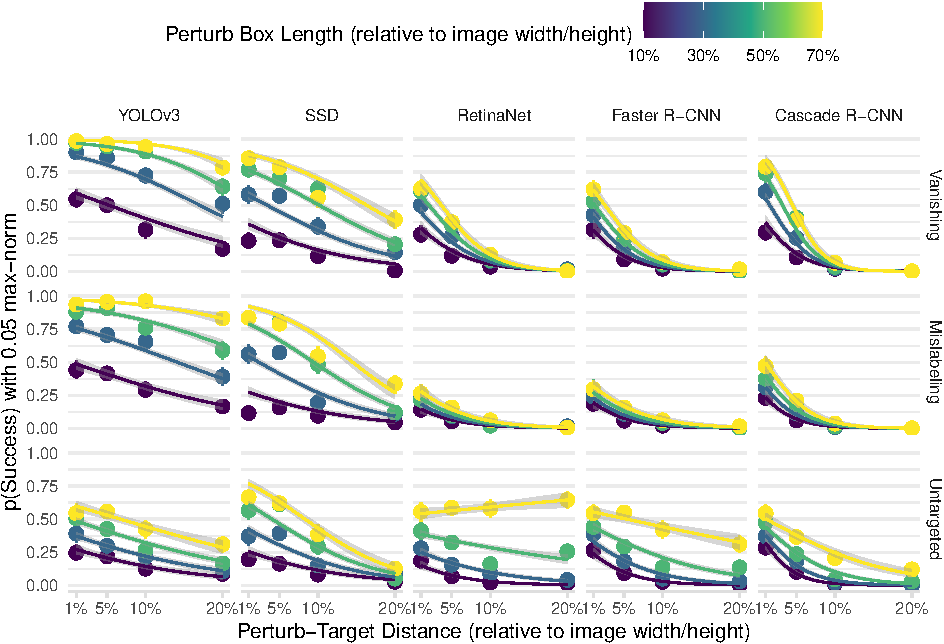
\includegraphics[width=1\linewidth]{rmd_imgs/arbitrary_trend_graph_normed} 

}

\caption{\textbf{A deliberate attack obfuscates intent with increased success for all models and attacks:}  We implement intent obfuscating attack by perturbing an arbitrary non-overlapping square region to disrupt a randomly selected target object at various lengths and distances. The binned summaries and regression trendlines graph success proportion against perturb-target distance (relative to image width/height) and perturb box length (relative to image width/height) in the deliberate attack experiment. Errors are 95\% confidence intervals.  and every point aggregates success over 200 images. The deliberate attack multiplies success as compared to the randomized attack (Figure \ref{fig:success_trend_graph}), especially at close perturb-target distance (relative to image width/height) and large perturb box length (relative to image width/height). Full details are given in Section \ref{sec:del_arb}.}\label{fig:arbitrary_trend_graph_normed}
\end{figure}

